
%%%%%%%%%%%%%%%%%%%%%%%%%%%%%%%%%%%%%%%%%%%%%%%%%%
\section{Data Quality}
%%%%%%%%%%%%%%%%%%%%%%%%%%%%%%%%%%%%%%%%%%%%%%%%%%
\subsection{Collected Data}

Table~\ref{Table:Data} shows list of the collected data while Oct/2010 Run.
800 MeV/$c$ pion is expected to pass-through the detector as MIP,
and have uniform energy deposition to all the TPC channels.
So this data set is very useful for calibrating the detector response (See section xxx).
800 MeV/$c$ proton stops after ~15 cm of flight distance inside the TPC fiducial volume
with relatively large $dE/dx$. So we use the proton data set for validation of the
detector response at high $dE/dx$ region(See section xxx).
We have collected three different Kaon data by varying thickness of the degrader. 
540, 630, 680 MeV/$c$ are corresponds to the momentum degraded by 
2 lead glass, 1 lead glass + 1 lead block, and 1 lead glass, respectively, 
and such Kaon stops after 10 cm, 50 cm, and 65 cm of flight distance inside TPC fiducial volume.

Figure~\ref{Fig:Textbook} shows an 2D display of typical event 
taken with 800 MeV/$c$ electron trigger.
Horizontal axis corresponds to TPC channel number 
and zero means most upper stream strip. 
Since strip pitch is 1 cm, this is equivalent to
distance from beam injection point in cm.
Vertical axis corresponds to electron drift time in $\mu$s
and t=0 means trigger timing. In this TPC, anode and cathode is
located at top and bottom of the detector, respectively,
t=0 means energy deposition at anode and longer drift time 
means energy deposition in lower height.
With 200 V/cm of electric field, drift velocity is about 0.8 m/ms.
So drift of full detector (40 cm) takes 500 $\mu$s.
Color strength of the plot corresponds to the TPC signal pulse height
in ADC counts which is roughly proportional to $dE/dx$ of the track.
In this event, triggered electron can be clearly seen center of the detector
as an electromagnetic shower while there are two other particles 
accidentally overlapped with the triggered electron. 
Track at t=100 $\mu$s is considered as
a proton which stops after 15 cm of flight distance and 
has large $dE/dx$ around the stopped point.
Track at t=400 $\mu$s is considered as
a pion which passes-through the detector and 
has uniform $dE/dx$ over the TPC channels.
This event already gives us some idea for how good 
the particle identification performance of the LArTPC is.

Figure~\ref{Fig:Kmunu} shows a typical $K \to\mu\nu$ like event.
We can clearly identify a kink of the track at 60 cm which is considered
as stopped point of Kaon and it decays to  

Energy deposition of the track is about MIP at the injection point
and gradually increase towards the stopped point at 60 cm.



\begin{table}[h]
\begin{center}
\caption{List of collected data}
\begin{tabular}{l|ll}
  Particle  &Momentum (MeV/$c$) &Number of Events\\
\hline
  Pion      &800                &3,000\\
  Proton    &800                &1,500\\
  Kaon      &540 (2LG)          &7,000\\
  Kaon      &630 (1LG+1LB)      &40,000\\
  Kaon      &680 (1LB)          &35,000\\
  electron  &800                &2,500\\
  electron  &200                &10,000\\
  pion      &200                &10,000\\
\end{tabular}
\label{Table:Data}
\end{center}
\end{table}



\begin{figure}[htbp]
 \begin{center}
  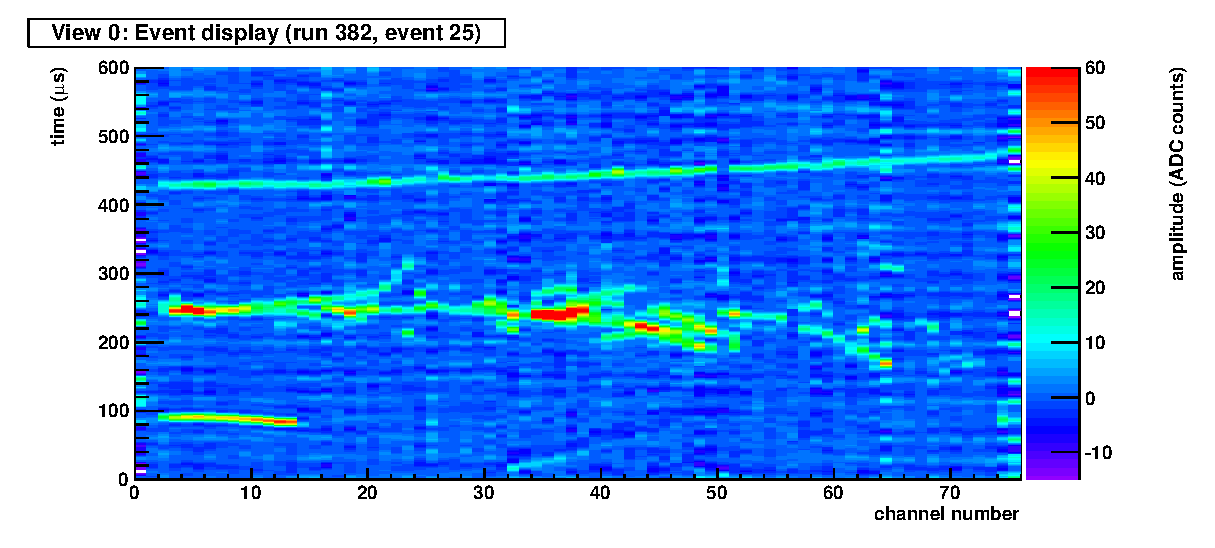
\includegraphics[width=100mm]{fig/Textbook.eps}
 \end{center}
 \caption{Event display of 800 MeV/$c$ electron triggered event.
Accidentally overlapped with a proton and a pion.}
 \label{Fig:Textbook}
\end{figure}

\begin{figure}[htbp]
 \begin{center}
  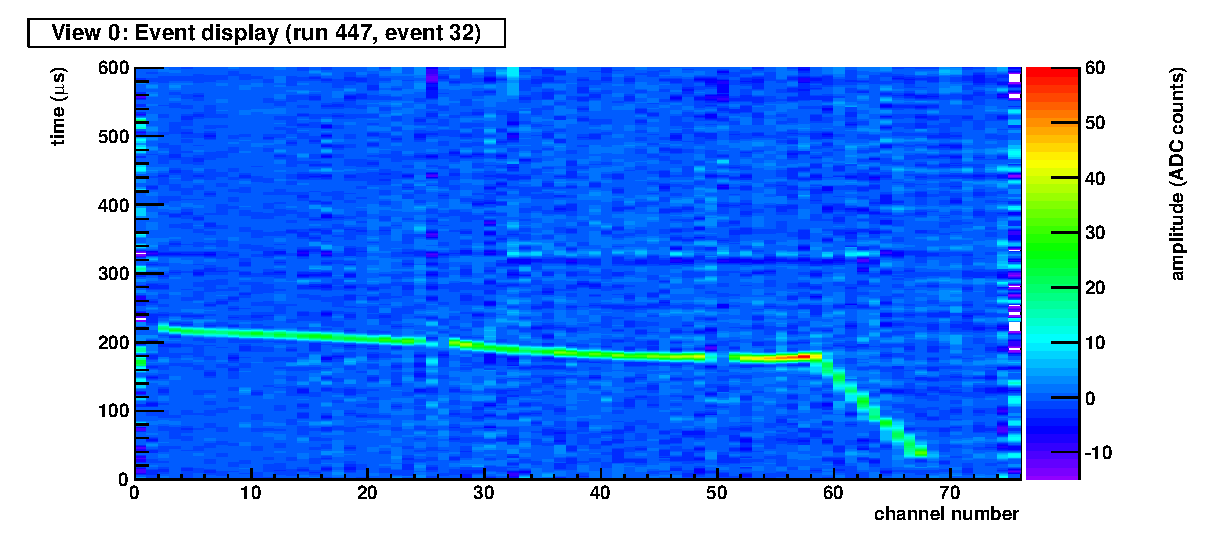
\includegraphics[width=100mm]{fig/Kmunu.eps}
 \end{center}
 \caption{Event display of Kaon 630 MeV/$c$ triggered event}
 \label{Fig:Kmunu}
\end{figure}

\subsection{Beam Quality (Purity)}
\begin{itemize}
\item Plot: TREK counters (FC, GC, TOF) (A. Okamoto)
\item Plot: TOF before and after selection  (A. Okamoto)
\end{itemize}

 As described in section xx, we have several beam counters
to identify beam particles event by event
Figure~ref{fig:TREK} shows response of the, FC, GC, and TOF counters.
By using these counter information,

\begin{table}[h]
\begin{tabular}{llll}
  Particle  &FC(K) &FC(pi) &GC\\
  Pion      &x     &o      &x\\
  Kaon      &o     &x      &x\\
  Proton    &o     &x      &x\\
  electron  &x     &o      &o\\

\end{tabular}
\caption{List of collected data}
\label{Table:Data}
\end{table}


GC is used to identify electrons
 
\subsection{Beam Energy, Position}
   \section{Beam Energy, Position}
   \subsection{Beam Energy}
 
   30GeV proton beam hits to target T1 in Hadron hall.
   It generates many particles like kaon, pion, muon, electron, and
   so on.
   We take the particles that has 800MeV/c momentum from this beam by
   using D1 magnet.\\
   \ \ For this analysis, a beam momentum at BDC after passing through the
   K1.1Br beam line is required.
   We estimate a beam momentum using simple MC simulation.
   Figure \ref{K11Br_Beam_line} shows MC simulation's geometory.
   This time, beam line is straight and has no electric and magnetic
   field.
   MC simulation shoot 800MeV/c kaon and pion as pencil beam.

   Figure \ref{k_pi_momentum} shows kaon and pion momentum distribution
   using this MC simulation.
   Actually, kaon momentum distribution peak is adjusted so that kaon
   decay point of MC simulation is consistent with data.
   Section \ref{kaon_energy_section} explains this point.
   And proton momentum is estimated in other way, using TREK detector
   TOF information.
   Section \ref{proton_energy_section} shows proton momentum distribution.

   \subsubsection{Kaon energy}\label{kaon_energy_section}

We adjust momentum peak of figure ?? and set Kaon beam energy  the point that the decay points of Kaon in data and simulation are good agreement. The distribution of decay poins are plotted in Figure\ref{DecayPoint_hough}.
\begin{figure}[!htb]
  \begin{center}
    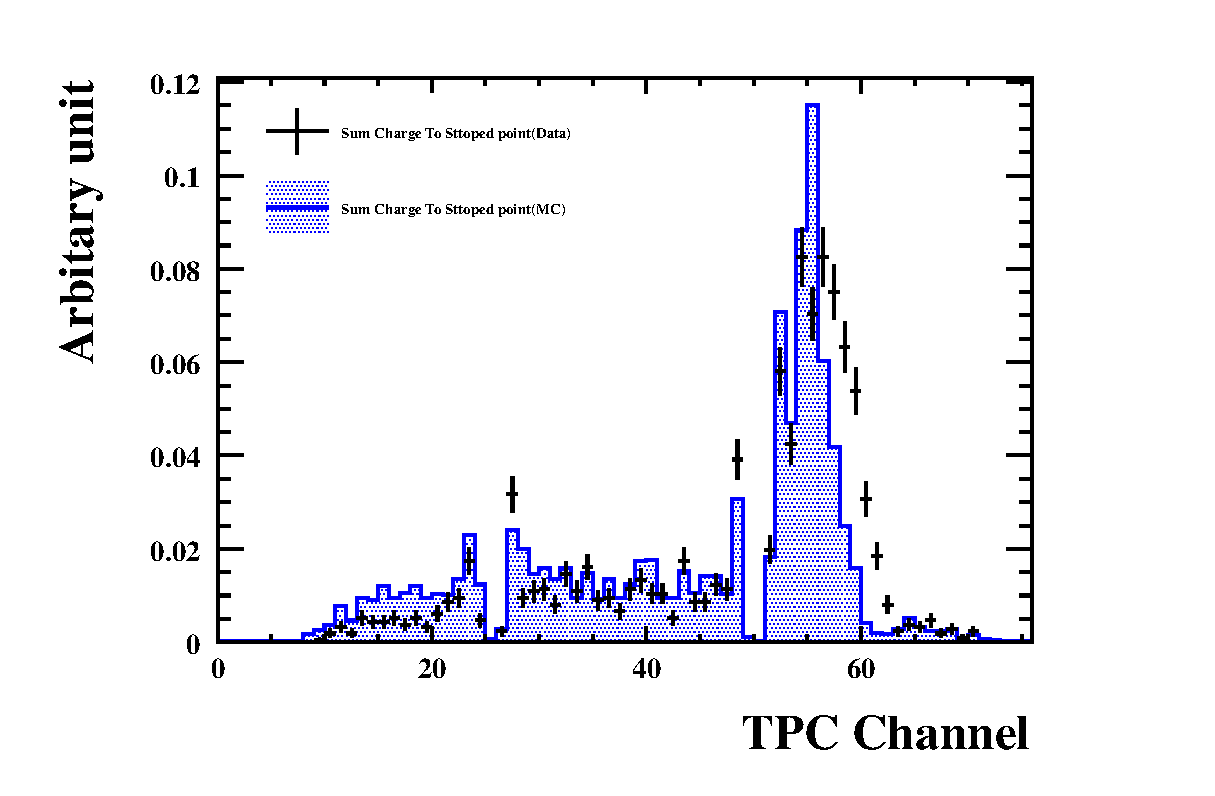
\includegraphics[width=70mm]{fig/cdp_hough.eps}
  \end{center}
  \caption{Decay point distribution of Data and MC}
  \label{DecayPoint_hough}
\end{figure}

   \subsubsection{Proton energy}\label{proton_energy_section}
   asuka




   \subsection{Energy deposition in degrader}
   Because of having high energy, kaon beam from BDC passes through 250LAr TPC.
   So that kaon stops in 250LAr TPC, we put degrader, which reduce
   beam energy, on beam line.
   In this experiment, we used lead glass and lead block as degrader.
   We estimate energy deposition in degrader by using MC simulation.
   Figure \ref{energy_deposition} shows energy deposition in degrader.
   
   \subsection{Beam Position}
   Before taking data, we measured a beam profile on the front of
   250LAr TPC by using plastic scintillation counter.
   Figure \ref{beamprofile_250L} shows beam profile on the front of
   250LAr TPC.

   \begin{figure}[!htb]
    \centering
    \centering
    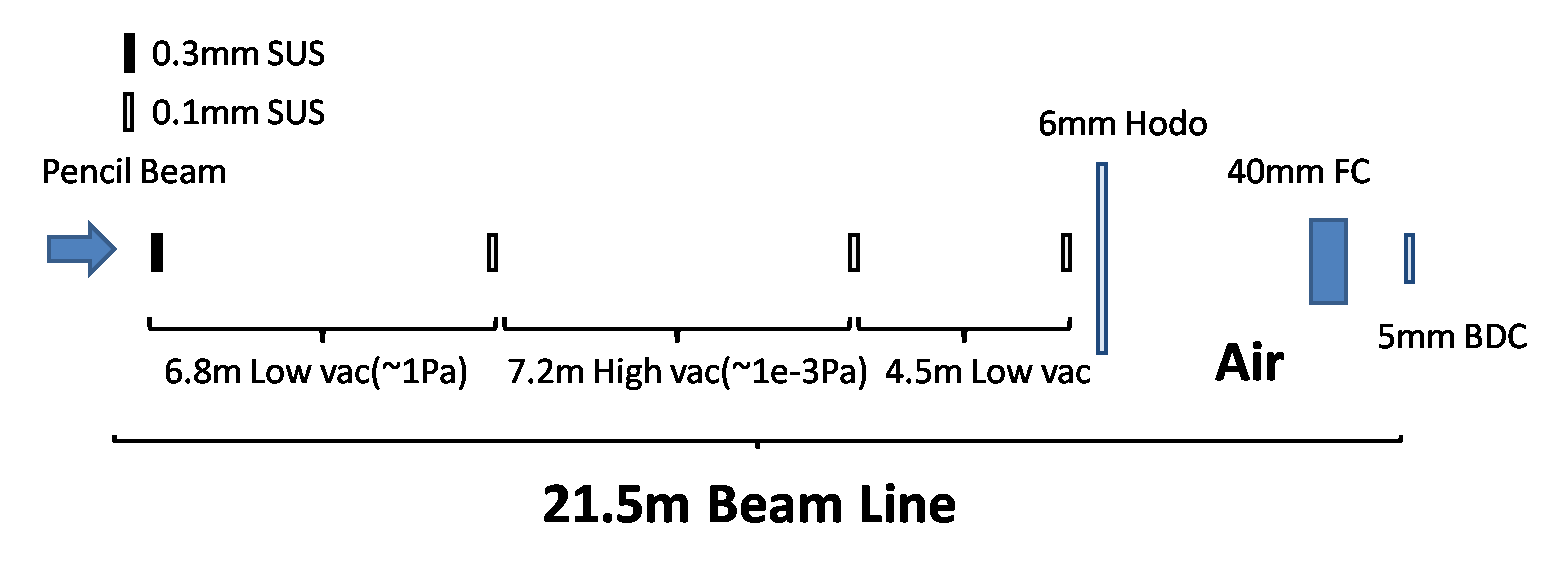
\includegraphics[width=11cm,clip]{./fig/K11Br_beamline_sim.eps}
    \caption{K1.1 Br beamline}
    \label{K11Br_Beam_line}
   \end{figure}



   \begin{figure}[!htb]
    \centering
    \centering
    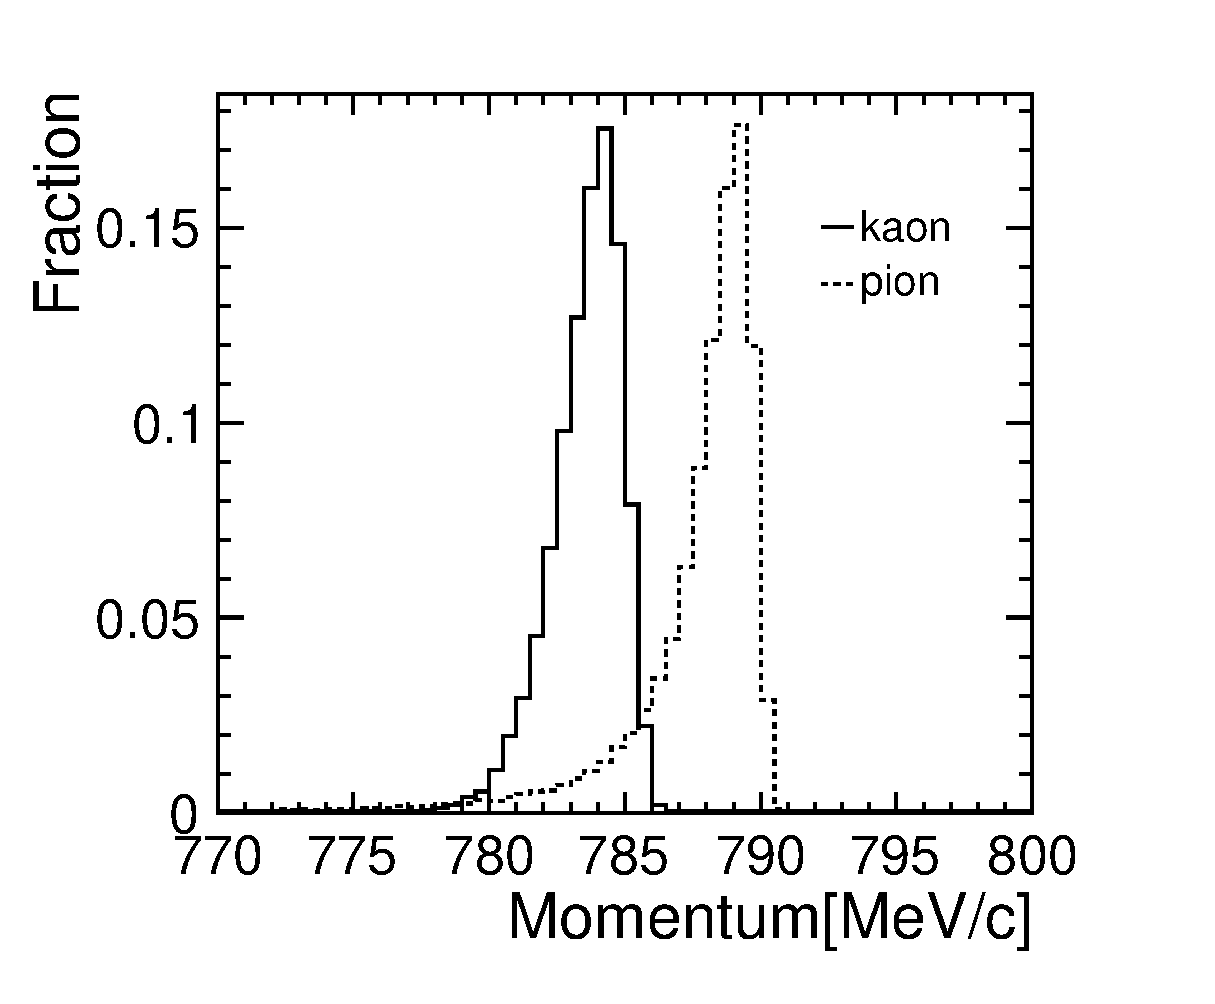
\includegraphics[width=11cm,clip]{./fig/Kaon_pion_momentum_nogrid.eps}
    \caption{kaon and pion momentum distribution at BDC}
    \label{k_pi_momentum}
   \end{figure}


   \begin{figure}[!htb]
    \centering
    \centering
    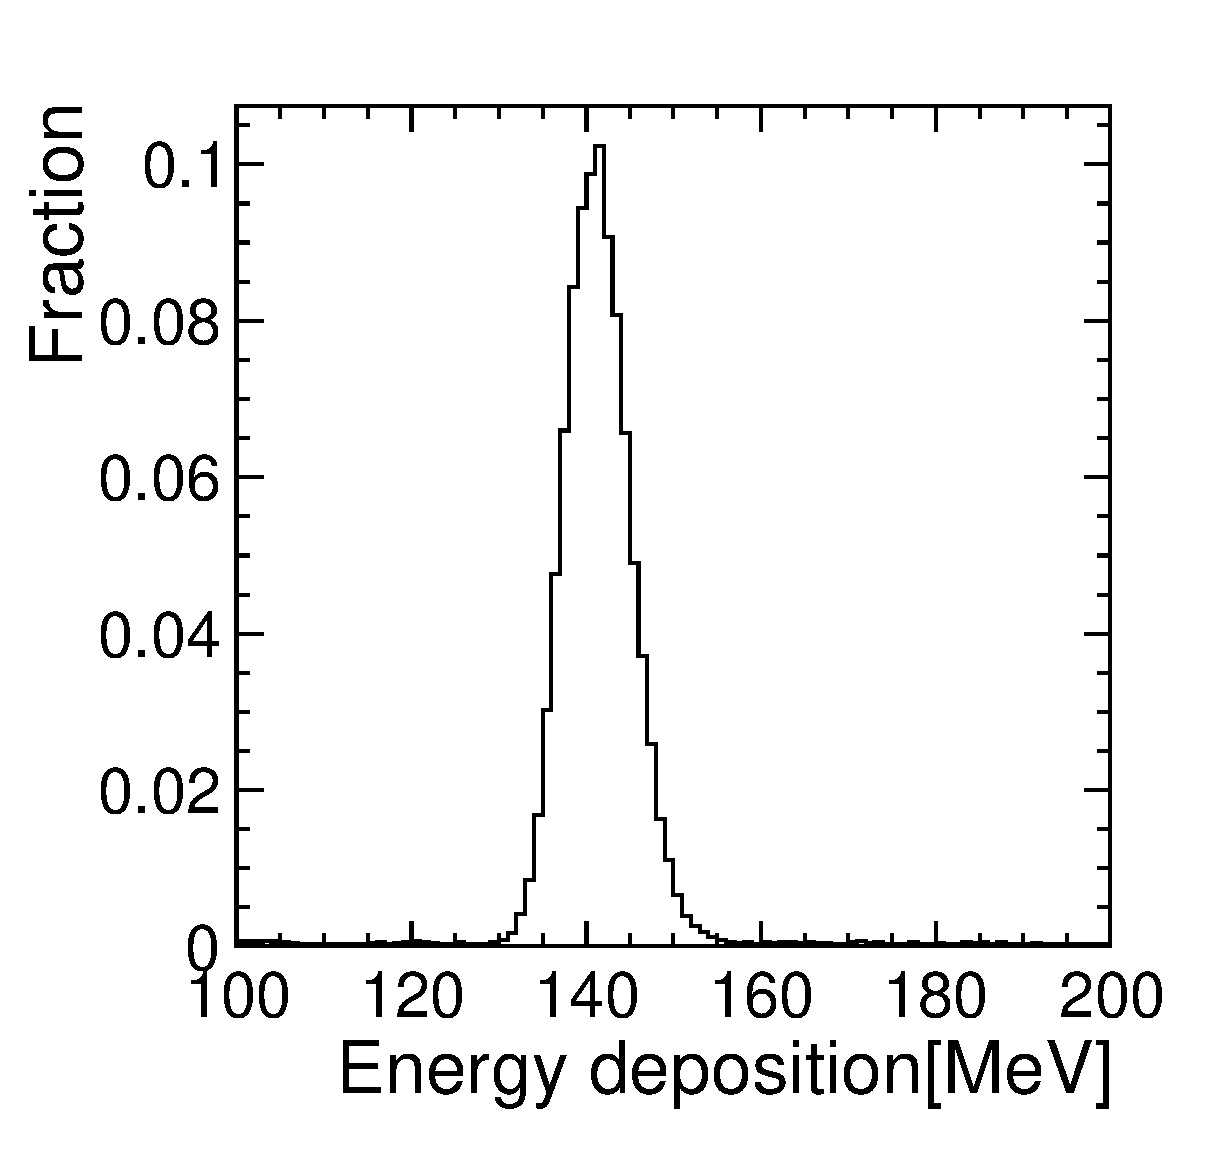
\includegraphics[width=11cm,clip]{./fig/energy_deposition.eps}
    \caption{energy deposition in degrader}
    \label{energy_deposition}
   \end{figure}


   \begin{figure}[!htb]
    \centering
    \centering
    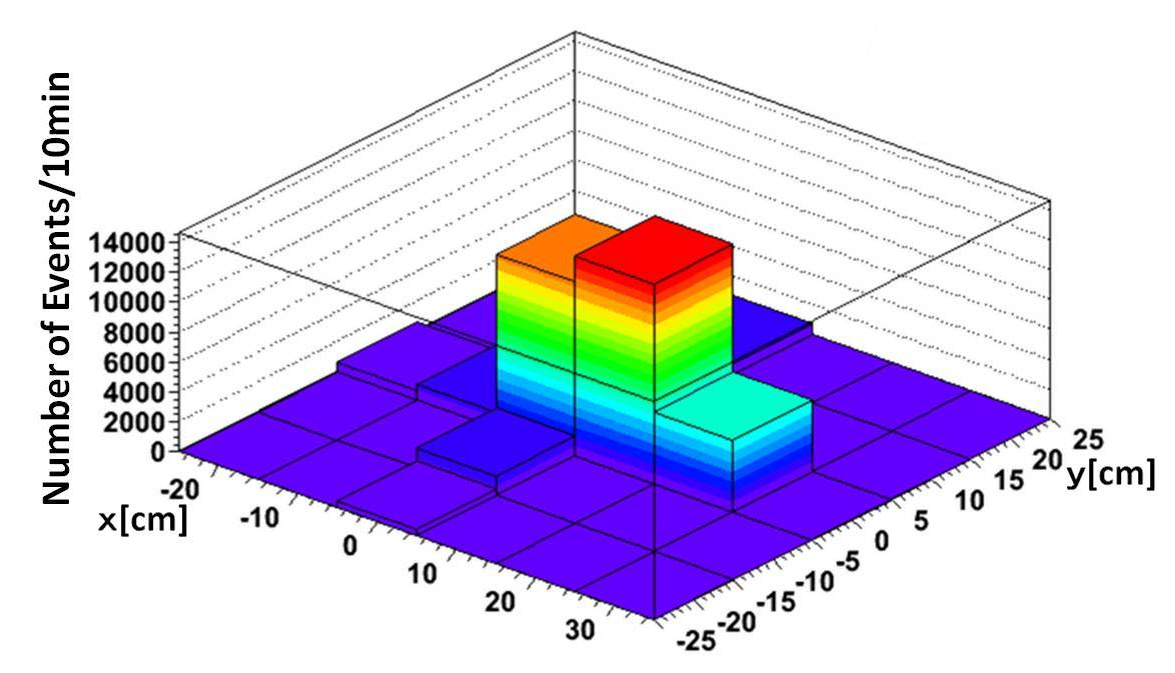
\includegraphics[width=11cm,clip]{./fig/BeamProfile3.eps}
    \caption{Beam profile on the front of 250LAr TPC}
    \label{beamprofile_250L}
   \end{figure}

\begin{itemize}
\item Plot: Proton momentum from TOF  (A. Okamoto)
\item Kaon:: Ongoing  (H. Okamoto?)
\item Plot: Beam position measurement
\end{itemize}

